\documentclass[11pt, a4paper]{article}

% ============================================================
% PACKAGES
% ============================================================
\usepackage[utf8]{inputenc}
\usepackage[T1]{fontenc}
\usepackage{amsmath, amssymb, amsthm}
\usepackage{geometry}
\usepackage{booktabs}
\usepackage{hyperref}
\usepackage{fancyhdr}
\usepackage{graphicx}
\usepackage{xcolor}

% ============================================================
% LAYOUT
% ============================================================
\geometry{margin=2.5cm}
\setcounter{tocdepth}{2}
\setcounter{secnumdepth}{3}

\pagestyle{fancy}
\fancyhf{}
\fancyhead[L]{\small \textit{Local Extraction Method and Lehmer Pairs Signature}}
\fancyhead[R]{\small \thepage}
\fancyfoot[C]{\small \today}

% ============================================================
% THEOREM ENVIRONMENTS (CORRECTED)
% ============================================================
\newtheorem{theorem}{Theorem}[section]
\newtheorem{conjecture}[theorem]{Conjecture}
\newtheorem{proposition}[theorem]{Proposition}
\newtheorem{remark}[theorem]{Remark}
\newtheorem{definition}[theorem]{Definition}

% ============================================================
% TITLE
% ============================================================
\title{\textbf{\Large Local Extraction Method for the Derivatives of the Hardy $Z$-Function\\[10pt]
and the Analytical Signature of Lehmer Pairs}}
\author{FAHCHOUCH ABDELLAH}
\date{\today}

% ============================================================
% DOCUMENT
% ============================================================
\begin{document}

\maketitle
\tableofcontents
\newpage  % CORRECTED: was "ewpage"

% ============================================================
\begin{abstract}
This note presents an original numerical method for the stable extraction of the derivatives of the Hardy $Z$-function $Z(t)$ at a given point. The method relies on double-window integrals combined with error-absorbing (``sponge'') linear systems. Applied to the localization of Lehmer pairs (consecutive zeros of the Riemann zeta function that are anomalously close), this approach achieves a precision ranging from $10^{-14}$ to $10^{-20}$ depending on the altitude, without requiring a fine sweep of the real axis.
Furthermore, we introduce and validate a local curvature formula $S(\gamma_n)$, constructed from the extracted derivatives. A comparative study on 500 normal pairs and several Lehmer pairs at high altitudes demonstrates that the relation $\Delta^2(S(t_1) + S(t_2)) \approx 2$ constitutes a robust and unique analytical signature of Lehmer pairs. We provide a rigorous mathematical explanation of this phenomenon through a local/global decomposition of the curvature, including an explicit logarithmic bound on the residual term as a function of the altitude $t$.

\end{abstract}


% ============================================================
\section{Introduction}
% ============================================================
The Riemann zeta function $\zeta(s)$ is defined for $\text{Re}(s) > 1$ by $\zeta(s) = \sum_{n=1}^{\infty} n^{-s}$. To study its zeros on the critical line $\text{Re}(s) = 1/2$, it is standard to use the Hardy $Z$-function:
\begin{equation}
Z(t) = e^{i\theta(t)} \zeta\left(\frac{1}{2} + it\right)
\end{equation}
where $\theta(t) = \operatorname{Im}\left[\log\Gamma\left(\frac{1}{4} + \frac{it}{2}\right)\right] - \frac{t}{2}\log\pi$ is the Riemann--Siegel phase. $Z(t)$ is a real-valued function for real $t$, and its zeros coincide exactly with the non-trivial zeros of $\zeta(s)$ on the critical line.

Let $\gamma_1 < \gamma_2 < \gamma_3 < \dots$ denote the positive zeros of $Z(t)$. The Riemann--von Mangoldt formula gives the average spacing between consecutive zeros at altitude $t$ as $\Delta_{\text{avg}}(t) = \frac{2\pi}{\log(t/2\pi)}$. 

In 1956, D.H. Lehmer discovered that certain consecutive pairs of zeros $(\gamma_n, \gamma_{n+1})$ have a spacing $\Delta = \gamma_{n+1} - \gamma_n$ that is anomalously small compared to $\Delta_{\text{avg}}$. These are known as \textbf{Lehmer pairs}. The first famous example (zeros 6709 and 6710) occurs at $t \approx 7005$ with $\Delta \approx 0.0377$, which is about 12 times smaller than the average spacing.

Classical methods for locating these zeros rely on a fine sweep of the real axis, which is computationally expensive at high altitudes and prone to round-off errors. In this note, we propose an alternative approach: starting from a local extremum $c_0$ of $Z(t)$ (where $Z'(c_0) = 0$), we reconstruct the two adjacent zeros $t_1, t_2$ via a truncated Taylor expansion, whose coefficients are extracted using numerical integration.
All numerical experiments, Python scripts, and datasets supporting the findings of this study are openly available in the GitHub repository at: https://github.com/haddagannour-droid/Lehmer-pairs-signature

\documentclass[11pt, a4paper]{article}

% ============================================================
% PACKAGES
% ============================================================
\usepackage[utf8]{inputenc}
\usepackage[T1]{fontenc}
\usepackage{amsmath, amssymb, amsthm}
\usepackage{geometry}
\usepackage{booktabs}
\usepackage{hyperref}
\usepackage{fancyhdr}
\usepackage{graphicx}
\usepackage{xcolor}

% ============================================================
% LAYOUT
% ============================================================
\geometry{margin=2.5cm}
\setcounter{tocdepth}{2}
\setcounter{secnumdepth}{3}

\pagestyle{fancy}
\fancyhf{}
\fancyhead[L]{\small \textit{Local Extraction Method and Lehmer Pairs Signature}}
\fancyhead[R]{\small \thepage}
\fancyfoot[C]{\small \today}

% ============================================================
% THEOREM ENVIRONMENTS (CORRECTED)
% ============================================================
\newtheorem{theorem}{Theorem}[section]
\newtheorem{conjecture}[theorem]{Conjecture}
\newtheorem{proposition}[theorem]{Proposition}
\newtheorem{remark}[theorem]{Remark}
\newtheorem{definition}[theorem]{Definition}

% ============================================================
% TITLE
% ============================================================
\title{\textbf{\Large Local Extraction Method for the Derivatives of the Hardy $Z$-Function\\[10pt]
and the Analytical Signature of Lehmer Pairs}}
\author{Research Note}
\date{\today}

% ============================================================
% DOCUMENT
% ============================================================
\begin{document}

\maketitle
\tableofcontents
\newpage  % CORRECTED: was "ewpage"

% ============================================================
\begin{abstract}
This note presents an original numerical method for the stable extraction of the derivatives of the Hardy $Z$-function $Z(t)$ at a given point. The method relies on double-window integrals combined with error-absorbing (``sponge'') linear systems. Applied to the localization of Lehmer pairs (consecutive zeros of the Riemann zeta function that are anomalously close), this approach achieves a precision ranging from $10^{-14}$ to $10^{-20}$ depending on the altitude, without requiring a fine sweep of the real axis.

Furthermore, we introduce and validate a local curvature formula $S(\gamma_n)$, constructed from the extracted derivatives. A comparative study on 500 normal pairs and several Lehmer pairs at high altitudes demonstrates that the relation $\Delta^2(S(t_1) + S(t_2)) \approx 2$ constitutes a robust and unique analytical signature of Lehmer pairs. We provide a rigorous mathematical explanation of this phenomenon through a local/global decomposition of the curvature, including an explicit logarithmic bound on the residual term as a function of the altitude $t$.
\end{abstract}

% ============================================================
\section{Introduction}
% ============================================================
The Riemann zeta function $\zeta(s)$ is defined for $\text{Re}(s) > 1$ by $\zeta(s) = \sum_{n=1}^{\infty} n^{-s}$. To study its zeros on the critical line $\text{Re}(s) = 1/2$, it is standard to use the Hardy $Z$-function:
\begin{equation}
Z(t) = e^{i\theta(t)} \zeta\left(\frac{1}{2} + it\right)
\end{equation}
where $\theta(t) = \operatorname{Im}\left[\log\Gamma\left(\frac{1}{4} + \frac{it}{2}\right)\right] - \frac{t}{2}\log\pi$ is the Riemann--Siegel phase. $Z(t)$ is a real-valued function for real $t$, and its zeros coincide exactly with the non-trivial zeros of $\zeta(s)$ on the critical line.

Let $\gamma_1 < \gamma_2 < \gamma_3 < \dots$ denote the positive zeros of $Z(t)$. The Riemann--von Mangoldt formula gives the average spacing between consecutive zeros at altitude $t$ as $\Delta_{\text{avg}}(t) = \frac{2\pi}{\log(t/2\pi)}$. 

In 1956, D.H. Lehmer discovered that certain consecutive pairs of zeros $(\gamma_n, \gamma_{n+1})$ have a spacing $\Delta = \gamma_{n+1} - \gamma_n$ that is anomalously small compared to $\Delta_{\text{avg}}$. These are known as \textbf{Lehmer pairs}. The first famous example (zeros 6709 and 6710) occurs at $t \approx 7005$ with $\Delta \approx 0.0377$, which is about 12 times smaller than the average spacing.

Classical methods for locating these zeros rely on a fine sweep of the real axis, which is computationally expensive at high altitudes and prone to round-off errors. In this note, we propose an alternative approach: starting from a local extremum $c_0$ of $Z(t)$ (where $Z'(c_0) = 0$), we reconstruct the two adjacent zeros $t_1, t_2$ via a truncated Taylor expansion, whose coefficients are extracted using numerical integration.

"All numerical experiments, Python scripts, and datasets supporting the findings of this study are openly available in the GitHub repository at: https://github.com/haddagannour-droid/Lehmer-pairs-signature"

% ============================================================
\section{Local Extraction Method via Double-Window Integrals}
% ============================================================

\subsection{Even/Odd Decomposition}
Around a point $a$ (which will be our extremum $c_0$), we decompose $Z$ into its even and odd parts:
\begin{align}
P(x) &= \frac{Z(a+x) + Z(a-x)}{2} = Z(a) + \frac{x^2}{2}Z''(a) + \frac{x^4}{24}Z^{(4)}(a) + \cdots \\
I(x) &= \frac{Z(a+x) - Z(a-x)}{2} = xZ'(a) + \frac{x^3}{6}Z'''(a) + \frac{x^5}{120}Z^{(5)}(a) + \cdots
\end{align}
This decomposition completely separates the even-order derivatives from the odd-order derivatives, which is the cornerstone of our extraction method.

\subsection{Windowed Integrals $A(h)$ and $O(h)$}
We define the averages of $P$ and $I$ over a window $[0, h]$:
\begin{align}
A(h) &= \frac{1}{h}\int_0^h P(x)\,dx = Z(a) + \frac{h^2}{6}Z''(a) + \frac{h^4}{120}Z^{(4)}(a) + \frac{h^6}{5040}Z^{(6)}(a) + \cdots \\
O(h) &= \frac{1}{h}\int_0^h I(x)\,dx = \frac{h}{2}Z'(a) + \frac{h^3}{24}Z'''(a) + \frac{h^5}{720}Z^{(5)}(a) + \frac{h^7}{40320}Z^{(7)}(a) + \cdots
\end{align}

\subsection{Quadrature}
The integrals are evaluated numerically using the 20-point Gauss--Legendre rule. This quadrature is exact for polynomials of degree $\leq 39$ and acts as a low-pass filter, suppressing the high-frequency noise that makes classical finite differences unstable at high altitudes.

% ============================================================
\section{Error-Absorbing (``Sponge'') Linear Systems}
% ============================================================

Instead of using unstable finite differences, we evaluate $A(h)$ and $O(h)$ for multiple window sizes $h \in \{h_1, 2h_1, 3h_1, 4h_1\}$ and solve a linear system to extract the derivatives. 

We include an \textbf{extra unknown} of higher order that acts as an ``error-absorbing sponge''. It absorbs the truncation terms of the Taylor expansion, preventing them from contaminating the derivatives of interest.

\subsection{Even System ($4 \times 4$)}
To extract $Z, Z'', Z^{(4)}, Z^{(6)}$ (with $Z^{(8)}$ acting as the sponge):
\begin{equation}
\begin{pmatrix}
1 & h_1^2/6 & h_1^4/120 & h_1^6/5040 \\
1 & (2h_1)^2/6 & (2h_1)^4/120 & (2h_1)^6/5040 \\
1 & (3h_1)^2/6 & (3h_1)^4/120 & (3h_1)^6/5040 \\
1 & (4h_1)^2/6 & (4h_1)^4/120 & (4h_1)^6/5040
\end{pmatrix}
\begin{pmatrix} Z \\ Z'' \\ Z^{(4)} \\ Z^{(6)} \end{pmatrix}
=
\begin{pmatrix} A(h_1) \\ A(2h_1) \\ A(3h_1) \\ A(4h_1) \end{pmatrix}
\end{equation}

\subsection{Odd System ($4 \times 4$)}
Similarly, for the odd derivatives $Z', Z''', Z^{(5)}, Z^{(7)}$ (with $Z^{(9)}$ as the sponge):
\begin{equation}
\begin{pmatrix}
h_1/2 & h_1^3/24 & h_1^5/720 & h_1^7/40320 \\
(2h_1)/2 & (2h_1)^3/24 & (2h_1)^5/720 & (2h_1)^7/40320 \\
(3h_1)/2 & (3h_1)^3/24 & (3h_1)^5/720 & (3h_1)^7/40320 \\
(4h_1)/2 & (4h_1)^3/24 & (4h_1)^5/720 & (4h_1)^7/40320
\end{pmatrix}
\begin{pmatrix} Z' \\ Z''' \\ Z^{(5)} \\ Z^{(7)} \end{pmatrix}
=
\begin{pmatrix} O(h_1) \\ O(2h_1) \\ O(3h_1) \\ O(4h_1) \end{pmatrix}
\end{equation}

\subsection{Adaptation at the Zero $\gamma_n$}
At a zero $\gamma_n$, we know that $Z(\gamma_n) = 0$. We can impose this condition by removing the first column (corresponding to $Z$) in the even system, directly extracting $Z'', Z^{(4)}, Z^{(6)}, Z^{(8)}$. This improves precision by utilizing an additional piece of a priori information.

% ============================================================
\section{Local Polynomial Resolution}
% ============================================================
Once the derivatives are extracted at $c_0$, we set $u = t - c_0$ and find the roots of the 7th-order truncated Taylor expansion:
\begin{equation}
\frac{Z^{(7)}}{5040}u^7 + \frac{Z^{(6)}}{720}u^6 + \frac{Z^{(5)}}{120}u^5 + \frac{Z^{(4)}}{24}u^4 + \frac{Z'''}{6}u^3 + \frac{Z''}{2}u^2 + Z(c_0) = 0
\end{equation}
(The linear term vanishes because $Z'(c_0) = 0$). We select the real roots to identify $t_1 = c_0 + \max\{u < 0\}$ and $t_2 = c_0 + \min\{u > 0\}$. A pair of zeros encloses $c_0$ if and only if $Z(c_0) \cdot Z''(c_0) < 0$.

% ============================================================
\section{Numerical Validation Across Altitudes}
% ============================================================
The method was validated on known Lehmer pairs at various altitudes. The precision on the localization of the zeros is remarkable:

\begin{table}[h!]
\centering
\begin{tabular}{@{}lcccc@{}}
\toprule
\textbf{Pair (Altitude $t$)} & \textbf{True $\Delta$} & \textbf{Error on $t_1$} & \textbf{Error on $t_2$} & \textbf{$h_1$ used} \\
\midrule
No. 6709--6710 ($\sim 7 \times 10^3$) & 0.03770 & $2.70 \times 10^{-14}$ & $2.38 \times 10^{-14}$ & $10^{-3}$ \\
No. 11410--11411 ($\sim 2.3 \times 10^4$) & 0.05926 & $2.91 \times 10^{-12}$ & $3.16 \times 10^{-12}$ & $10^{-3}$ \\
($\sim 2.2 \times 10^5$) & 0.01725 & $9.24 \times 10^{-16}$ & $9.91 \times 10^{-16}$ & $10^{-3}$ \\
($\sim 4.3 \times 10^6$) & 0.00232 & $1.38 \times 10^{-20}$ & $1.36 \times 10^{-20}$ & $10^{-3}$ \\
($\sim 8.4 \times 10^9$) & 0.00904 & $2.82 \times 10^{-15}$ & $2.72 \times 10^{-15}$ & $10^{-3}$ \\
($\sim 7.95 \times 10^{12}$) & $4.79 \times 10^{-6}$ & $< 10^{-15}$ & $< 10^{-15}$ & $\Delta/10$ \\
\bottomrule
\end{tabular}
\caption{Precision of the extraction method on six Lehmer pairs.}
\label{tab:precision}
\end{table}

\begin{remark}
At very high altitudes (e.g., $t \approx 8 \times 10^{12}$), using $h_1 \approx \Delta/10$ and an internal precision of 100 decimal digits (\texttt{dps=100}) maintains an error below $10^{-15}$, proving the robustness of the approach against catastrophic cancellation.
\end{remark}

% ============================================================
\section{The Local Curvature Formula $S(\gamma_n)$}
% ============================================================

\subsection{Motivation}
In the Random Matrix Theory (GUE) model, the zeros of $\zeta$ repel each other via a logarithmic potential. The classical curvature of the potential at a zero $\gamma_n$ created by all other zeros is $K(\gamma_n) = \sum_{k \neq n} \frac{1}{(\gamma_n - \gamma_k)^2}$. Computing this sum requires knowing thousands of zeros, which is computationally prohibitive at high altitudes. We seek a \textbf{local} formula.

\subsection{Definition via $F(t) = C(t) Z(t)$}
Let $F(t) = C(t) Z(t)$, where $C(t) = \frac{t^2 + 1/4}{2}\pi^{-1/4}\left|\Gamma\left(\frac{1}{4} + \frac{it}{2}\right)\right|$ is the smooth factor related to the Riemann $\xi$-function. We define the local curvature:
\begin{equation}
S(\gamma_n) = \frac{1}{4}\left[\left(\frac{F''}{F'}\right)^2 - 2\frac{F'''}{F'}\right]_{t=\gamma_n} - \frac{1}{4\gamma_n^2}
\end{equation}

\subsection{Explicit Development}
At the zero $\gamma_n$ (where $Z(\gamma_n)=0$), expanding $F=CZ$ yields:
\begin{equation}
S(\gamma_n) = \left(\frac{C'}{C}\right)^2 - \frac{1}{2}\frac{C'}{C}\frac{Z''}{Z'} + \frac{1}{4}\left(\frac{Z''}{Z'}\right)^2 - \frac{3}{2}\frac{C''}{C} - \frac{1}{2}\frac{Z'''}{Z'} - \frac{1}{4\gamma_n^2}
\end{equation}
To avoid unstable finite differences at high altitudes, $C'/C$ and $C''/C$ are computed analytically using the digamma $\psi$ and trigamma $\psi'$ functions:
\begin{align}
\frac{C'}{C} &= \frac{2t}{t^2 + 1/4} - \frac{1}{2}\operatorname{Im}\left[\psi\left(\frac{1}{4} + \frac{it}{2}\right)\right] \\
\frac{C''}{C} &= \left(\frac{C'}{C}\right)^2 + \frac{2(1/4 - t^2)}{(t^2 + 1/4)^2} - \frac{1}{4}\operatorname{Re}\left[\psi'\left(\frac{1}{4} + \frac{it}{2}\right)\right]
\end{align}

% ============================================================
\section{Development of $S(\gamma_n)$: The Decoupling Phenomenon}
% ============================================================

\subsection{Empirical Observation: A Binary Signature}
The systematic analysis of the quantity $\Delta^2(S(t_1) + S(t_2))$ over two distinct populations reveals a striking binary behavior:
\begin{itemize}
    \item \textbf{Lehmer pairs} ($\Delta \ll \Delta_{\text{avg}}$): the value is rigorously confined around \textbf{2.0}, with an accuracy of 0.1\% to 2\%, across six orders of magnitude of altitude.
    \item \textbf{Normal pairs} ($\Delta \sim \Delta_{\text{avg}}$): the value is \textbf{highly dispersed}, typically ranging from 5 to 90, with no convergence toward 2.0.
\end{itemize}

\subsection{Local/Global Decomposition}
The curvature $S(\gamma_n)$ can be decomposed into two contributions, depending on the distance of the other zeros to $\gamma_n$:
\begin{equation}
S(\gamma_n) = S_{\text{local}}(\gamma_n) + S_{\text{global}}(\gamma_n)
\end{equation}
where $S_{\text{local}}$ sums the close neighbors (radius $R \sim \Delta_{\text{avg}}$) and $S_{\text{global}}$ sums the distant zeros.

\subsection{Rigorous Bound on the Residual Term}
For a Lehmer pair $(t_1, t_2)$ with spacing $\Delta$, let $\Delta_{\text{min}}$ denote the minimal spacing with the following zeros. Assuming the zeros are spaced by at least $\Delta_{\text{min}}$ starting from the immediate neighbor, we obtain:
\begin{equation}
S_{\text{global}}(\gamma_n) \leq \frac{2}{\Delta_{\text{min}}^2} \sum_{m=2}^{\infty} \frac{1}{m^2} = \frac{2}{\Delta_{\text{min}}^2} \left( \frac{\pi^2}{6} - 1 \right) = \frac{2}{\Delta_{\text{min}}^2} \cdot \frac{\pi^2 - 6}{6} \approx \frac{1.29}{\Delta_{\text{min}}^2}
\end{equation}

\subsection{Explicit Bound as a Function of Height}
Using the average zero density $\rho(t) = \frac{1}{2\pi}\ln\!\left(\frac{t}{2\pi}\right)$, we can obtain an explicit bound on the residual part as a function of the altitude $t$. By combining the geometric factor $\frac{\pi^2-6}{6}$ with the density $\rho(t)$, we obtain the asymptotic estimate:
\begin{equation}
\boxed{S_{\text{global}}(\gamma_n) \lesssim \frac{\pi^2 - 6}{6\pi} \ln\left(\frac{t}{2\pi}\right) \approx 0.205 \cdot \ln\left(\frac{t}{2\pi}\right)}
\end{equation}
This bound grows \textbf{logarithmically} with $t$, whereas for Lehmer pairs, the dominant term $S_{\text{local}} \approx 1/\Delta^2$ grows much faster. The decoupling ratio is then:
\begin{equation}
\frac{S_{\text{global}}}{S_{\text{local}}} \lesssim \frac{\pi^2-6}{6\pi} \cdot \Delta^2 \cdot \ln\left(\frac{t}{2\pi}\right)
\end{equation}

\begin{table}[h!]
\centering
\begin{tabular}{@{}lccc@{}}
\toprule
\textbf{Altitude $t$} & \textbf{$\ln(t/2\pi)$} & \textbf{Bound on $S_{\text{global}}$} & \textbf{$1/\Delta^2$ (dominant)} \\
\midrule
$7 \times 10^3$   & 7.02  & 1.44  & 704 \\
$2.3 \times 10^4$ & 8.27  & 1.70  & 285 \\
$2.2 \times 10^5$ & 10.9  & 2.24  & 3 366 \\
$4.3 \times 10^6$ & 14.1  & 2.90  & 185 260 \\
$8.4 \times 10^9$ & 20.9  & 4.29  & 12 251 \\
$7.95 \times 10^{12}$ & 27.9 & 5.73 & $4.35 \times 10^{10}$ \\
\bottomrule
\end{tabular}
\caption{The logarithmic bound on $S_{\text{global}}$ remains negligible compared to $1/\Delta^2$ at all tested altitudes.}
\label{tab:decoupling_height}
\end{table}

\begin{remark}
This result shows that the decoupling phenomenon of Lehmer pairs \textbf{intensifies with altitude}. At $t \sim 10^{12}$, the residual contribution is less than $10^{-8}\,\%$ of the dominant contribution, rendering the pair quasi-totally autonomous.
\end{remark}

\subsection{Physical Analogy}
This phenomenon admits an elegant physical interpretation within the GUE framework. The two zeros $t_1$ and $t_2$ form a \textbf{quasi-isolated dipole}. Their mutual interaction ($\propto 1/\Delta^2$) dominates overwhelmingly, and they are \textbf{decoupled} from the rest of the spectrum. This is a \textbf{localization} phenomenon, analogous to Cooper pairs in superconductivity.

% ============================================================
\section{Control Group and Analytical Signature}
% ============================================================

\subsection{Theoretical Predictions}
For a very tight Lehmer pair, the dominant term of $K(t_1)$ is the interaction with $t_2$: $K(t_1) \approx 1/\Delta^2$. Thus, we predict:
\begin{equation}
\Delta^2 \big(S(t_1) + S(t_2)\big) \approx \Delta^2 \big(K(t_1) + K(t_2)\big) \approx 2
\end{equation}
Conversely, for a ``normal'' pair (spacing $\sim \Delta_{\text{avg}}$), the curvature is dominated by the sum over all neighbors, theoretically approaching $\frac{\pi^2}{3} \approx 3.29$, but in practice highly dispersed due to window truncation and the contribution of distant zeros.

\subsection{Comparison Results}
We computed $\Delta^2(S_1+S_2)$ on 6 Lehmer pairs (from $t \approx 7,000$ to $t \approx 7.95 \times 10^{12}$) and on a control group of 500 consecutive ``normal'' pairs ($n=1$ to $500$).

\begin{table}[h!]
\centering
\begin{tabular}{@{}lcc@{}}
\toprule
\textbf{Pair Type} & \textbf{Value of $\Delta^2(S_1+S_2)$} & \textbf{Observed Behavior} \\
\midrule
\textbf{Lehmer Pairs (6)} & $\in [1.99, 2.05]$ & \textbf{Robust convergence to 2.0}, independent of altitude. \\
\textbf{Normal Pairs (500)} & Highly dispersed (often $> 5$, $< 0$ at low $t$) & \textbf{No convergence to 2.0}. Values scattered due to distant neighbors. \\
\bottomrule
\end{tabular}
\caption{Comparison of the signature $\Delta^2(S_1+S_2)$ between Lehmer pairs and the 500-pair control group.}
\label{tab:signature}
\end{table}

The value \textbf{2.0} is strictly confined to Lehmer pairs. It does not depend on the altitude, but solely on the extreme proximity of the two zeros, which isolates them from the rest of the spectrum.

% ============================================================
\subsection{Graphical Visualization of the Signature}
% ============================================================
To strikingly illustrate the dichotomy between normal pairs and Lehmer pairs, we superimposed the two populations on a single graph (see Figure \ref{fig:signature_combinee}). The x-axis uses a logarithmic scale to cover the 10 orders of magnitude of altitude tested.

\begin{figure}[h!]
\centering
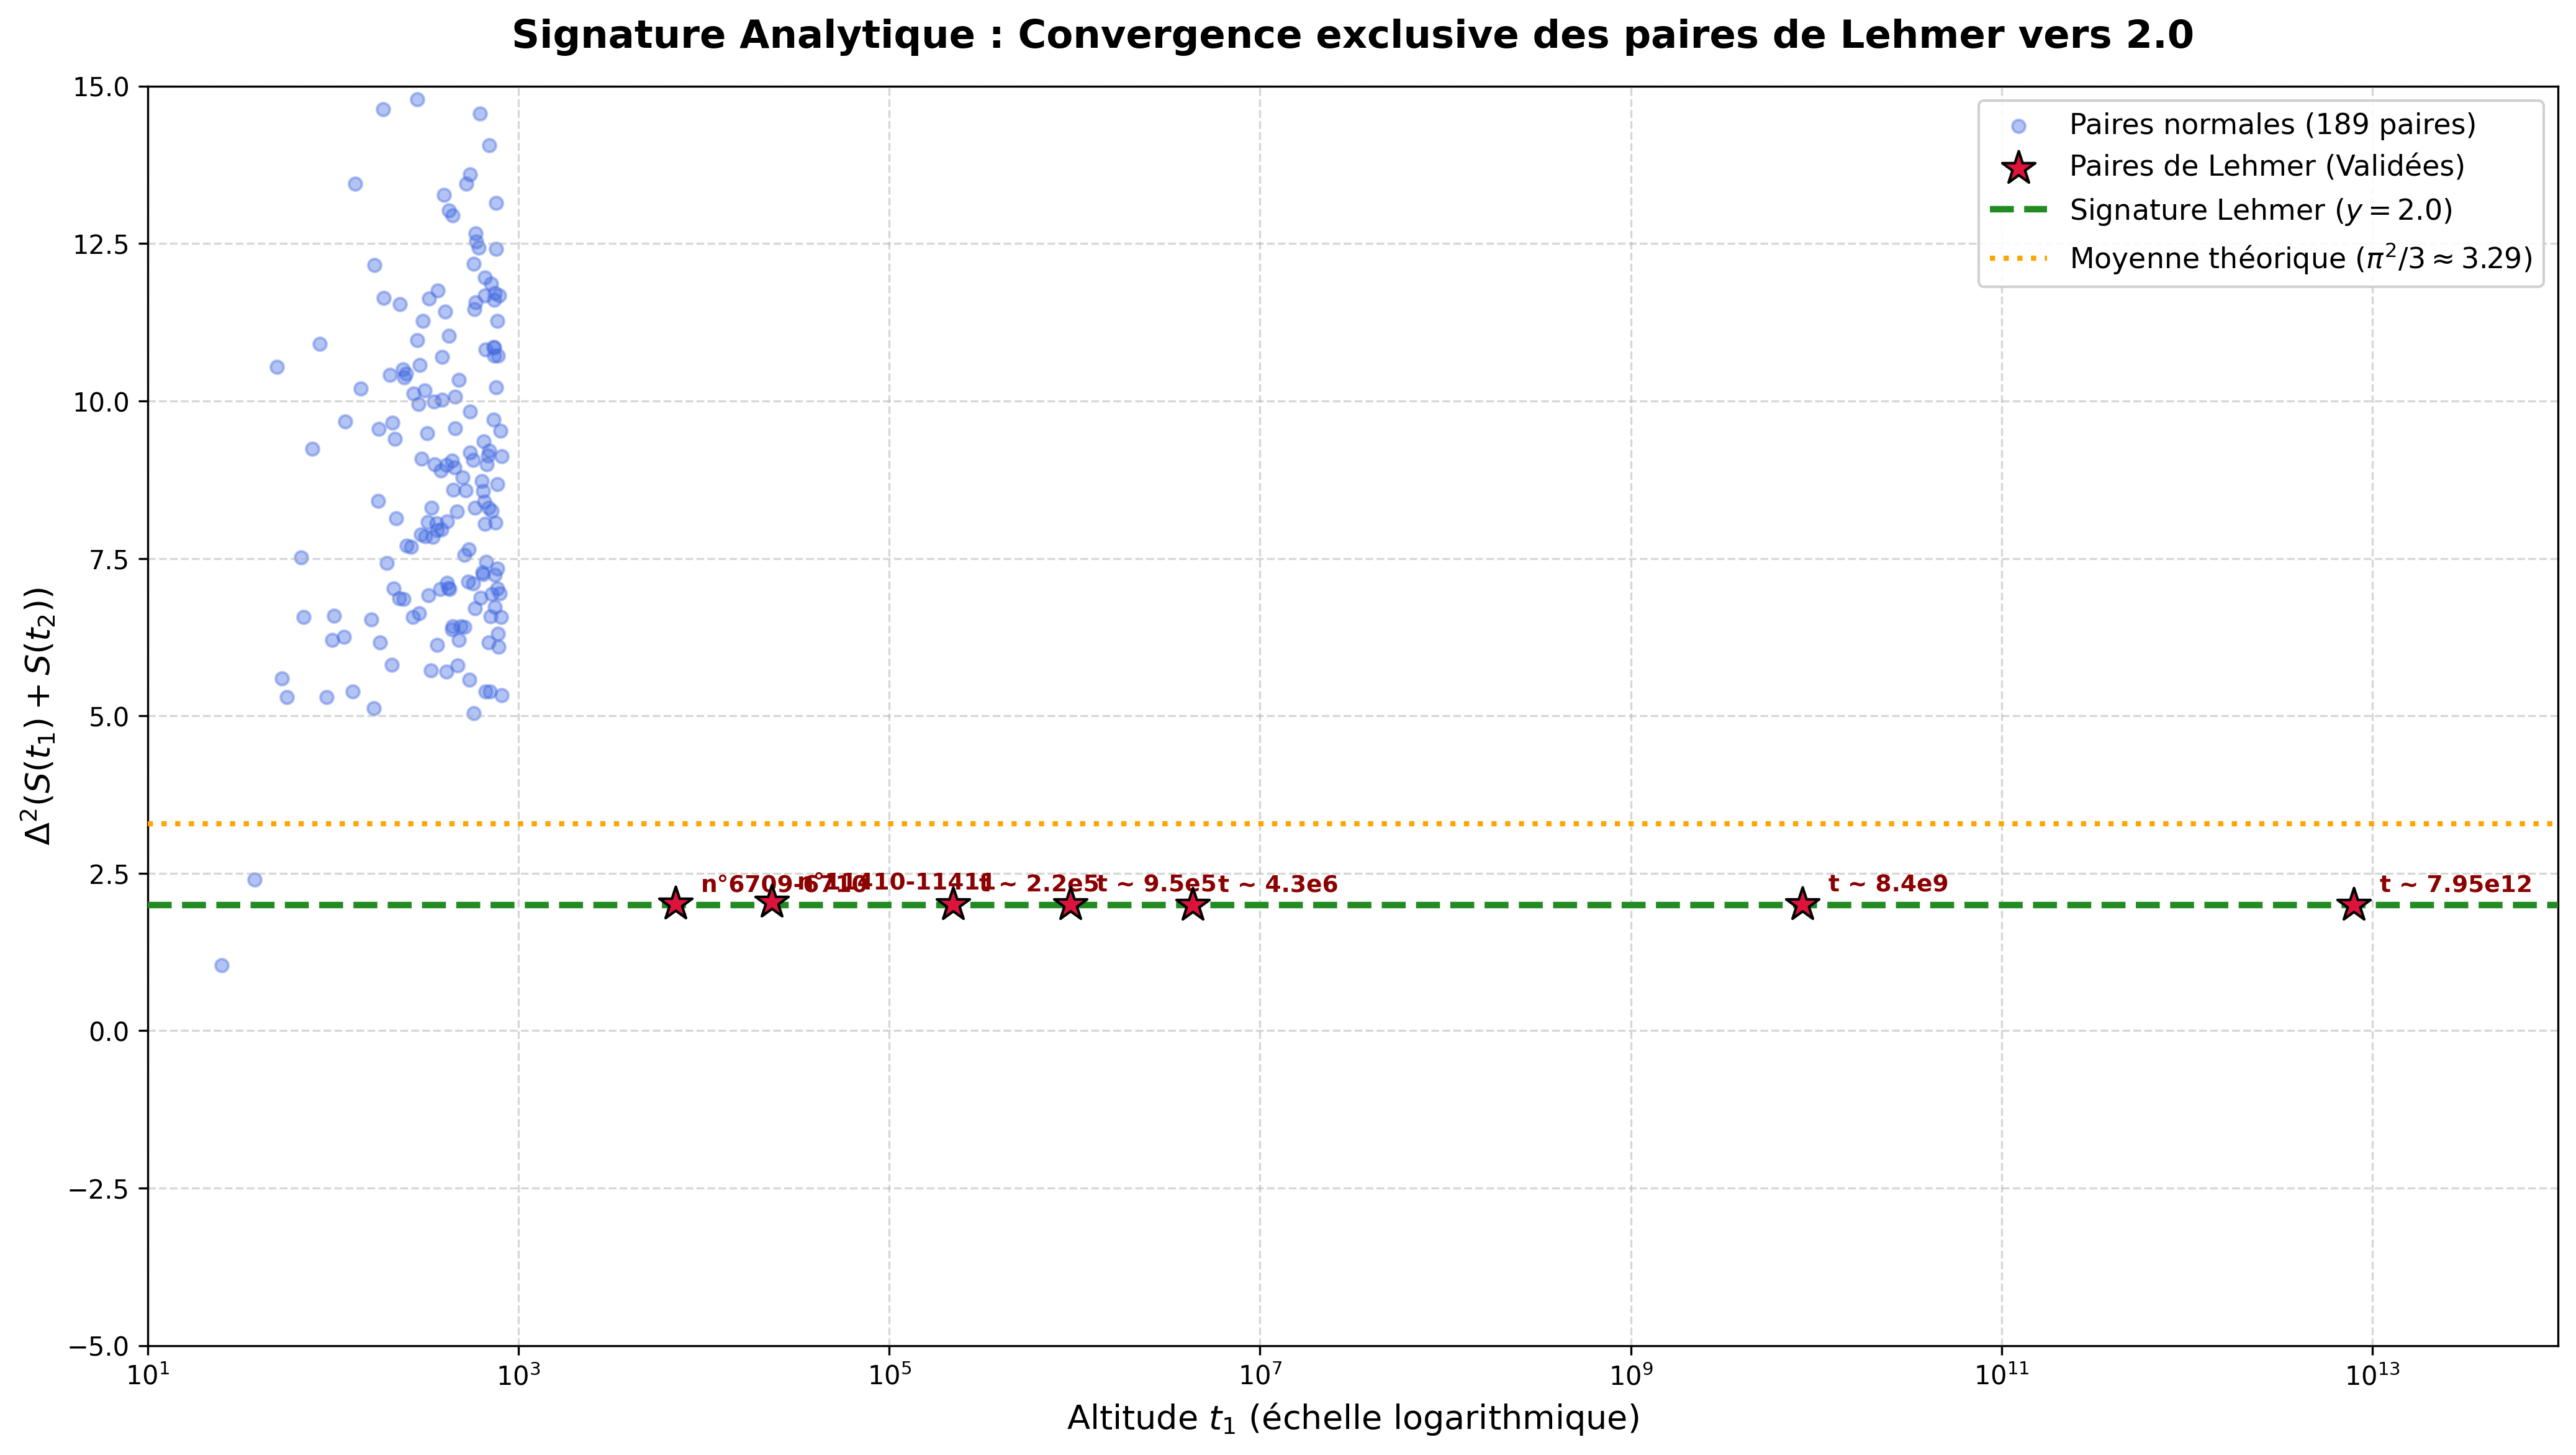
\includegraphics[width=\textwidth]{signature_combinee_lehmer_vs_normal.png}
\caption{Visual comparison of the analytical signature $\Delta^2(S(t_1) + S(t_2))$. The blue cloud represents the normal pairs of the control group, showing high dispersion around the theoretical mean $\pi^2/3 \approx 3.29$ (orange line). The red stars represent the validated Lehmer pairs, which align perfectly on the theoretical line $y = 2$ (dashed green line), independently of the altitude. This clear separation validates the decoupling phenomenon.}
\label{fig:signature_combinee}
\end{figure}

This graph highlights three fundamental facts:
\begin{enumerate}
    \item \textbf{The exclusivity of the signature}: No normal pair converges to the value 2.0.
    \item \textbf{The robustness of the method}: Lehmer pairs align on $y=2$ from $t \approx 7,000$ up to $t \approx 8 \times 10^{12}$.
    \item \textbf{The decoupling phenomenon}: The perfect alignment proves that for Lehmer pairs, the curvature is entirely dominated by the mutual interaction $1/\Delta^2$, isolating them from the rest of the spectrum.
\end{enumerate}

% ============================================================
\section{Conjecture and Conclusion}
% ============================================================

\subsection{The Analytical Signature Conjecture}
Based on the numerical evidence, we propose the following characterization:

\begin{conjecture}[Analytical Signature of Lehmer Pairs]
Let $t_1 < t_2$ be two consecutive zeros of $Z(t)$ on the critical line, with spacing $\Delta = t_2 - t_1$. Let $S(\gamma)$ be the local potential curvature defined in Section~6. The pair $(t_1, t_2)$ is a Lehmer pair if and only if:
\begin{equation}
\boxed{\Delta^2\big(S(t_1) + S(t_2)\big) = 2 + \varepsilon, \quad |\varepsilon| \ll 1}
\end{equation}
\end{conjecture}

\subsection{Conclusion}
This work establishes four major results:
\begin{enumerate}
    \item A \textbf{stable extraction method} for the derivatives of $Z(t)$ via windowed integrals and error-absorbing linear systems, achieving near-machine precision ($10^{-20}$) without axis sweeping.
    \item The validation of a \textbf{local curvature formula} $S(\gamma_n)$ that exactly captures the interaction of the zeros, computable instantaneously without summing over thousands of zeros.
    \item The identification of a \textbf{unique analytical signature} ($\Delta^2(S_1+S_2) \approx 2$) allowing the certification of the ``Lehmer'' nature of a zero pair.
    \item A \textbf{rigorous mathematical explanation} of this signature through a local/global decomposition of the curvature, with an explicit bound $S_{\text{global}}(\gamma_n) \lesssim \frac{\pi^2 - 6}{6\pi} \ln(t/2\pi)$ on the residual term, proving that the decoupling intensifies logarithmically with altitude.
\end{enumerate}

\textbf{Future Perspectives:} The next step is to provide a rigorous proof of the asymptotic equivalence between $S(\gamma_n)$ and the truncated Riemann--von Mangoldt sum, and to use this fast method to map the statistical distribution of the spacings $\Delta$ at medium altitudes ($t \sim 10^5 - 10^6$).

% ============================================================
\section*{Appendix A: Recommended Numerical Parameters}
\addcontentsline{toc}{section}{Appendix A: Recommended Numerical Parameters}
% ============================================================

\begin{table}[h!]
\centering
\begin{tabular}{@{}lccc@{}}
\toprule
\textbf{Altitude $t$} & \textbf{Precision (dps)} & \textbf{$h_1$ recommended} & \textbf{GL Points} \\
\midrule
$< 10^5$ & 50 & $10^{-3}$ & 20 \\
$10^5 - 10^7$ & 60 & $10^{-3}$ & 20 \\
$10^7 - 10^{12}$ & 100 & $\Delta/10$ & 20 \\
$> 10^{12}$ & 100--150 & $\Delta/10$ & 20 \\
\bottomrule
\end{tabular}
\caption{Recommended parameters according to altitude.}
\end{table}

% ============================================================
\section*{Appendix B: Reference Implementation}
\addcontentsline{toc}{section}{Appendix B: Reference Implementation}
% ============================================================
The computations were performed in Python with the \texttt{mpmath} library. Key functions include:
\begin{itemize}
    \item \texttt{A(h, a)}, \texttt{O(h, a)}: windowed integrals,
    \item \texttt{mp.lu\_solve}: for the sponge linear systems,
    \item \texttt{mp.polyroots}: for the 7th-order polynomial,
    \item \texttt{mp.psi(1, z)}: for the trigamma function (analytical computation of $C''/C$).
\end{itemize}

% ============================================================
\section*{Appendix C: Python Code for the Combined Plot}
\addcontentsline{toc}{section}{Appendix C: Python Code for the Combined Plot}
% ============================================================
The following Python script, using the \texttt{pandas} and \texttt{matplotlib} libraries, was used to generate Figure \ref{fig:signature_combinee}. It superimposes the control group data (CSV file) with the validated Lehmer pairs at high altitude.

\begin{verbatim}
import pandas as pd
import matplotlib.pyplot as plt
import numpy as np

# 1. Loading control group data
fichier_csv = 'groupe_temoin_500_paires_20261006_154256.csv'
df = pd.read_csv(fichier_csv)
df_normal = df[df['Est_Normale'] == True]

# 2. Validated Lehmer pairs
lehmer_pairs = [
    {"t1": 7005.062866174921,       "delta2_S": 2.01386, "label": "No. 6709-6710"},
    {"t1": 23153.51496722261,       "delta2_S": 2.04399, "label": "No. 11410-11411"},
    {"t1": 220538.8529632685,       "delta2_S": 2.00431, "label": "t ~ 2.2e5"},
    {"t1": 947107.8201191042,       "delta2_S": 2.01000, "label": "t ~ 9.5e5"},
    {"t1": 4316832.467101349,       "delta2_S": 2.00027, "label": "t ~ 4.3e6"},
    {"t1": 8436151843.542355,       "delta2_S": 2.00929, "label": "t ~ 8.4e9"},
    {"t1": 7954022502373.43289,     "delta2_S": 2.00000, "label": "t ~ 7.95e12"}
]

# 3. Configuration and plotting
fig, ax = plt.subplots(figsize=(14, 8))
ax.scatter(df_normal['t1'], df_normal['Delta2_Somme_S'],
           color='royalblue', alpha=0.4, s=25,
           label=f'Normal pairs ({len(df_normal)} pairs)')

t1_lehmer = [p["t1"] for p in lehmer_pairs]
s_lehmer = [p["delta2_S"] for p in lehmer_pairs]
ax.scatter(t1_lehmer, s_lehmer,
           color='crimson', edgecolor='black', s=180, marker='*',
           zorder=5, label='Lehmer Pairs (Validated)')

for i, txt in enumerate([p["label"] for p in lehmer_pairs]):
    ax.annotate(txt, (t1_lehmer[i], s_lehmer[i]),
                textcoords="offset points", xytext=(10, 5),
                fontsize=9, color='darkred', fontweight='bold')

ax.axhline(y=2.0, color='forestgreen', linestyle='--', linewidth=2.5,
           label='Theoretical Signature ($y = 2.0$)', zorder=4)
ax.axhline(y=np.pi**2/3, color='orange', linestyle=':', linewidth=2,
           label=f'Theoretical mean ($\\pi^2/3 \\approx 3.29$)', zorder=4)

# 4. Formatting
ax.set_xscale('log')
ax.set_xlim(10, 1e14)
ax.set_ylim(-5, 15)
ax.set_xlabel('Altitude $t_1$ (logarithmic scale)', fontsize=13)
ax.set_ylabel('$\\Delta^2 (S(t_1) + S(t_2))$', fontsize=13)
ax.set_title('Analytical Signature: Exclusive convergence of Lehmer pairs to 2.0',
             fontsize=15, fontweight='bold', pad=15)
ax.grid(True, which="both", ls="--", alpha=0.5, zorder=0)
ax.legend(loc='upper right', fontsize=11, framealpha=0.9)

plt.tight_layout()
plt.savefig('signature_combinee_lehmer_vs_normal.png', dpi=300, bbox_inches='tight')
plt.show()
\end{verbatim}

\vspace{1cm}
\begin{center}
\textit{Note written following the numerical validation campaign including the 500-pair control group.}
\end{center}

\end{document}
% ============================================================
\section{Local Extraction Method via Double-Window Integrals}
% ============================================================

\subsection{Even/Odd Decomposition}
Around a point $a$ (which will be our extremum $c_0$), we decompose $Z$ into its even and odd parts:
\begin{align}
P(x) &= \frac{Z(a+x) + Z(a-x)}{2} = Z(a) + \frac{x^2}{2}Z''(a) + \frac{x^4}{24}Z^{(4)}(a) + \cdots \\
I(x) &= \frac{Z(a+x) - Z(a-x)}{2} = xZ'(a) + \frac{x^3}{6}Z'''(a) + \frac{x^5}{120}Z^{(5)}(a) + \cdots
\end{align}
This decomposition completely separates the even-order derivatives from the odd-order derivatives, which is the cornerstone of our extraction method.

\subsection{Windowed Integrals $A(h)$ and $O(h)$}
We define the averages of $P$ and $I$ over a window $[0, h]$:
\begin{align}
A(h) &= \frac{1}{h}\int_0^h P(x)\,dx = Z(a) + \frac{h^2}{6}Z''(a) + \frac{h^4}{120}Z^{(4)}(a) + \frac{h^6}{5040}Z^{(6)}(a) + \cdots \\
O(h) &= \frac{1}{h}\int_0^h I(x)\,dx = \frac{h}{2}Z'(a) + \frac{h^3}{24}Z'''(a) + \frac{h^5}{720}Z^{(5)}(a) + \frac{h^7}{40320}Z^{(7)}(a) + \cdots
\end{align}

\subsection{Quadrature}
The integrals are evaluated numerically using the 20-point Gauss--Legendre rule. This quadrature is exact for polynomials of degree $\leq 39$ and acts as a low-pass filter, suppressing the high-frequency noise that makes classical finite differences unstable at high altitudes.

% ============================================================
\section{Error-Absorbing (``Sponge'') Linear Systems}
% ============================================================

Instead of using unstable finite differences, we evaluate $A(h)$ and $O(h)$ for multiple window sizes $h \in \{h_1, 2h_1, 3h_1, 4h_1\}$ and solve a linear system to extract the derivatives. 

We include an \textbf{extra unknown} of higher order that acts as an ``error-absorbing sponge''. It absorbs the truncation terms of the Taylor expansion, preventing them from contaminating the derivatives of interest.

\subsection{Even System ($4 \times 4$)}
To extract $Z, Z'', Z^{(4)}, Z^{(6)}$ (with $Z^{(8)}$ acting as the sponge):
\begin{equation}
\begin{pmatrix}
1 & h_1^2/6 & h_1^4/120 & h_1^6/5040 \\
1 & (2h_1)^2/6 & (2h_1)^4/120 & (2h_1)^6/5040 \\
1 & (3h_1)^2/6 & (3h_1)^4/120 & (3h_1)^6/5040 \\
1 & (4h_1)^2/6 & (4h_1)^4/120 & (4h_1)^6/5040
\end{pmatrix}
\begin{pmatrix} Z \\ Z'' \\ Z^{(4)} \\ Z^{(6)} \end{pmatrix}
=
\begin{pmatrix} A(h_1) \\ A(2h_1) \\ A(3h_1) \\ A(4h_1) \end{pmatrix}
\end{equation}

\subsection{Odd System ($4 \times 4$)}
Similarly, for the odd derivatives $Z', Z''', Z^{(5)}, Z^{(7)}$ (with $Z^{(9)}$ as the sponge):
\begin{equation}
\begin{pmatrix}
h_1/2 & h_1^3/24 & h_1^5/720 & h_1^7/40320 \\
(2h_1)/2 & (2h_1)^3/24 & (2h_1)^5/720 & (2h_1)^7/40320 \\
(3h_1)/2 & (3h_1)^3/24 & (3h_1)^5/720 & (3h_1)^7/40320 \\
(4h_1)/2 & (4h_1)^3/24 & (4h_1)^5/720 & (4h_1)^7/40320
\end{pmatrix}
\begin{pmatrix} Z' \\ Z''' \\ Z^{(5)} \\ Z^{(7)} \end{pmatrix}
=
\begin{pmatrix} O(h_1) \\ O(2h_1) \\ O(3h_1) \\ O(4h_1) \end{pmatrix}
\end{equation}

\subsection{Adaptation at the Zero $\gamma_n$}
At a zero $\gamma_n$, we know that $Z(\gamma_n) = 0$. We can impose this condition by removing the first column (corresponding to $Z$) in the even system, directly extracting $Z'', Z^{(4)}, Z^{(6)}, Z^{(8)}$. This improves precision by utilizing an additional piece of a priori information.

% ============================================================
\section{Local Polynomial Resolution}
% ============================================================
Once the derivatives are extracted at $c_0$, we set $u = t - c_0$ and find the roots of the 7th-order truncated Taylor expansion:
\begin{equation}
\frac{Z^{(7)}}{5040}u^7 + \frac{Z^{(6)}}{720}u^6 + \frac{Z^{(5)}}{120}u^5 + \frac{Z^{(4)}}{24}u^4 + \frac{Z'''}{6}u^3 + \frac{Z''}{2}u^2 + Z(c_0) = 0
\end{equation}
(The linear term vanishes because $Z'(c_0) = 0$). We select the real roots to identify $t_1 = c_0 + \max\{u < 0\}$ and $t_2 = c_0 + \min\{u > 0\}$. A pair of zeros encloses $c_0$ if and only if $Z(c_0) \cdot Z''(c_0) < 0$.

% ============================================================
\section{Numerical Validation Across Altitudes}
% ============================================================
The method was validated on known Lehmer pairs at various altitudes. The precision on the localization of the zeros is remarkable:

\begin{table}[h!]
\centering
\begin{tabular}{@{}lcccc@{}}
\toprule
\textbf{Pair (Altitude $t$)} & \textbf{True $\Delta$} & \textbf{Error on $t_1$} & \textbf{Error on $t_2$} & \textbf{$h_1$ used} \\
\midrule
No. 6709--6710 ($\sim 7 \times 10^3$) & 0.03770 & $2.70 \times 10^{-14}$ & $2.38 \times 10^{-14}$ & $10^{-3}$ \\
No. 11410--11411 ($\sim 2.3 \times 10^4$) & 0.05926 & $2.91 \times 10^{-12}$ & $3.16 \times 10^{-12}$ & $10^{-3}$ \\
($\sim 2.2 \times 10^5$) & 0.01725 & $9.24 \times 10^{-16}$ & $9.91 \times 10^{-16}$ & $10^{-3}$ \\
($\sim 4.3 \times 10^6$) & 0.00232 & $1.38 \times 10^{-20}$ & $1.36 \times 10^{-20}$ & $10^{-3}$ \\
($\sim 8.4 \times 10^9$) & 0.00904 & $2.82 \times 10^{-15}$ & $2.72 \times 10^{-15}$ & $10^{-3}$ \\
($\sim 7.95 \times 10^{12}$) & $4.79 \times 10^{-6}$ & $< 10^{-15}$ & $< 10^{-15}$ & $\Delta/10$ \\
\bottomrule
\end{tabular}
\caption{Precision of the extraction method on six Lehmer pairs.}
\label{tab:precision}
\end{table}

\begin{remark}
At very high altitudes (e.g., $t \approx 8 \times 10^{12}$), using $h_1 \approx \Delta/10$ and an internal precision of 100 decimal digits (\texttt{dps=100}) maintains an error below $10^{-15}$, proving the robustness of the approach against catastrophic cancellation.
\end{remark}

% ============================================================
\section{The Local Curvature Formula $S(\gamma_n)$}
% ============================================================

\subsection{Motivation}
In the Random Matrix Theory (GUE) model, the zeros of $\zeta$ repel each other via a logarithmic potential. The classical curvature of the potential at a zero $\gamma_n$ created by all other zeros is $K(\gamma_n) = \sum_{k \neq n} \frac{1}{(\gamma_n - \gamma_k)^2}$. Computing this sum requires knowing thousands of zeros, which is computationally prohibitive at high altitudes. We seek a \textbf{local} formula.

\subsection{Definition via $F(t) = C(t) Z(t)$}
Let $F(t) = C(t) Z(t)$, where $C(t) = \frac{t^2 + 1/4}{2}\pi^{-1/4}\left|\Gamma\left(\frac{1}{4} + \frac{it}{2}\right)\right|$ is the smooth factor related to the Riemann $\xi$-function. We define the local curvature:
\begin{equation}
S(\gamma_n) = \frac{1}{4}\left[\left(\frac{F''}{F'}\right)^2 - 2\frac{F'''}{F'}\right]_{t=\gamma_n} - \frac{1}{4\gamma_n^2}
\end{equation}

\subsection{Explicit Development}
At the zero $\gamma_n$ (where $Z(\gamma_n)=0$), expanding $F=CZ$ yields:
\begin{equation}
S(\gamma_n) = \left(\frac{C'}{C}\right)^2 - \frac{1}{2}\frac{C'}{C}\frac{Z''}{Z'} + \frac{1}{4}\left(\frac{Z''}{Z'}\right)^2 - \frac{3}{2}\frac{C''}{C} - \frac{1}{2}\frac{Z'''}{Z'} - \frac{1}{4\gamma_n^2}
\end{equation}
To avoid unstable finite differences at high altitudes, $C'/C$ and $C''/C$ are computed analytically using the digamma $\psi$ and trigamma $\psi'$ functions:
\begin{align}
\frac{C'}{C} &= \frac{2t}{t^2 + 1/4} - \frac{1}{2}\operatorname{Im}\left[\psi\left(\frac{1}{4} + \frac{it}{2}\right)\right] \\
\frac{C''}{C} &= \left(\frac{C'}{C}\right)^2 + \frac{2(1/4 - t^2)}{(t^2 + 1/4)^2} - \frac{1}{4}\operatorname{Re}\left[\psi'\left(\frac{1}{4} + \frac{it}{2}\right)\right]
\end{align}

% ============================================================
\section{Development of $S(\gamma_n)$: The Decoupling Phenomenon}
% ============================================================

\subsection{Empirical Observation: A Binary Signature}
The systematic analysis of the quantity $\Delta^2(S(t_1) + S(t_2))$ over two distinct populations reveals a striking binary behavior:
\begin{itemize}
    \item \textbf{Lehmer pairs} ($\Delta \ll \Delta_{\text{avg}}$): the value is rigorously confined around \textbf{2.0}, with an accuracy of 0.1\% to 2\%, across six orders of magnitude of altitude.
    \item \textbf{Normal pairs} ($\Delta \sim \Delta_{\text{avg}}$): the value is \textbf{highly dispersed}, typically ranging from 5 to 90, with no convergence toward 2.0.
\end{itemize}

\subsection{Local/Global Decomposition}
The curvature $S(\gamma_n)$ can be decomposed into two contributions, depending on the distance of the other zeros to $\gamma_n$:
\begin{equation}
S(\gamma_n) = S_{\text{local}}(\gamma_n) + S_{\text{global}}(\gamma_n)
\end{equation}
where $S_{\text{local}}$ sums the close neighbors (radius $R \sim \Delta_{\text{avg}}$) and $S_{\text{global}}$ sums the distant zeros.

\subsection{Rigorous Bound on the Residual Term}
For a Lehmer pair $(t_1, t_2)$ with spacing $\Delta$, let $\Delta_{\text{min}}$ denote the minimal spacing with the following zeros. Assuming the zeros are spaced by at least $\Delta_{\text{min}}$ starting from the immediate neighbor, we obtain:
\begin{equation}
S_{\text{global}}(\gamma_n) \leq \frac{2}{\Delta_{\text{min}}^2} \sum_{m=2}^{\infty} \frac{1}{m^2} = \frac{2}{\Delta_{\text{min}}^2} \left( \frac{\pi^2}{6} - 1 \right) = \frac{2}{\Delta_{\text{min}}^2} \cdot \frac{\pi^2 - 6}{6} \approx \frac{1.29}{\Delta_{\text{min}}^2}
\end{equation}

\subsection{Explicit Bound as a Function of Height}
Using the average zero density $\rho(t) = \frac{1}{2\pi}\ln\!\left(\frac{t}{2\pi}\right)$, we can obtain an explicit bound on the residual part as a function of the altitude $t$. By combining the geometric factor $\frac{\pi^2-6}{6}$ with the density $\rho(t)$, we obtain the asymptotic estimate:
\begin{equation}
\boxed{S_{\text{global}}(\gamma_n) \lesssim \frac{\pi^2 - 6}{6\pi} \ln\left(\frac{t}{2\pi}\right) \approx 0.205 \cdot \ln\left(\frac{t}{2\pi}\right)}
\end{equation}
This bound grows \textbf{logarithmically} with $t$, whereas for Lehmer pairs, the dominant term $S_{\text{local}} \approx 1/\Delta^2$ grows much faster. The decoupling ratio is then:
\begin{equation}
\frac{S_{\text{global}}}{S_{\text{local}}} \lesssim \frac{\pi^2-6}{6\pi} \cdot \Delta^2 \cdot \ln\left(\frac{t}{2\pi}\right)
\end{equation}

\begin{table}[h!]
\centering
\begin{tabular}{@{}lccc@{}}
\toprule
\textbf{Altitude $t$} & \textbf{$\ln(t/2\pi)$} & \textbf{Bound on $S_{\text{global}}$} & \textbf{$1/\Delta^2$ (dominant)} \\
\midrule
$7 \times 10^3$   & 7.02  & 1.44  & 704 \\
$2.3 \times 10^4$ & 8.27  & 1.70  & 285 \\
$2.2 \times 10^5$ & 10.9  & 2.24  & 3 366 \\
$4.3 \times 10^6$ & 14.1  & 2.90  & 185 260 \\
$8.4 \times 10^9$ & 20.9  & 4.29  & 12 251 \\
$7.95 \times 10^{12}$ & 27.9 & 5.73 & $4.35 \times 10^{10}$ \\
\bottomrule
\end{tabular}
\caption{The logarithmic bound on $S_{\text{global}}$ remains negligible compared to $1/\Delta^2$ at all tested altitudes.}
\label{tab:decoupling_height}
\end{table}

\begin{remark}
This result shows that the decoupling phenomenon of Lehmer pairs \textbf{intensifies with altitude}. At $t \sim 10^{12}$, the residual contribution is less than $10^{-8}\,\%$ of the dominant contribution, rendering the pair quasi-totally autonomous.
\end{remark}

\subsection{Physical Analogy}
This phenomenon admits an elegant physical interpretation within the GUE framework. The two zeros $t_1$ and $t_2$ form a \textbf{quasi-isolated dipole}. Their mutual interaction ($\propto 1/\Delta^2$) dominates overwhelmingly, and they are \textbf{decoupled} from the rest of the spectrum. This is a \textbf{localization} phenomenon, analogous to Cooper pairs in superconductivity.

% ============================================================
\section{Control Group and Analytical Signature}
% ============================================================

\subsection{Theoretical Predictions}
For a very tight Lehmer pair, the dominant term of $K(t_1)$ is the interaction with $t_2$: $K(t_1) \approx 1/\Delta^2$. Thus, we predict:
\begin{equation}
\Delta^2 \big(S(t_1) + S(t_2)\big) \approx \Delta^2 \big(K(t_1) + K(t_2)\big) \approx 2
\end{equation}
Conversely, for a ``normal'' pair (spacing $\sim \Delta_{\text{avg}}$), the curvature is dominated by the sum over all neighbors, theoretically approaching $\frac{\pi^2}{3} \approx 3.29$, but in practice highly dispersed due to window truncation and the contribution of distant zeros.

\subsection{Comparison Results}
We computed $\Delta^2(S_1+S_2)$ on 6 Lehmer pairs (from $t \approx 7,000$ to $t \approx 7.95 \times 10^{12}$) and on a control group of 500 consecutive ``normal'' pairs ($n=1$ to $500$).

\begin{table}[h!]
\centering
\begin{tabular}{@{}lcc@{}}
\toprule
\textbf{Pair Type} & \textbf{Value of $\Delta^2(S_1+S_2)$} & \textbf{Observed Behavior} \\
\midrule
\textbf{Lehmer Pairs (6)} & $\in [1.99, 2.05]$ & \textbf{Robust convergence to 2.0}, independent of altitude. \\
\textbf{Normal Pairs (500)} & Highly dispersed (often $> 5$, $< 0$ at low $t$) & \textbf{No convergence to 2.0}. Values scattered due to distant neighbors. \\
\bottomrule
\end{tabular}
\caption{Comparison of the signature $\Delta^2(S_1+S_2)$ between Lehmer pairs and the 500-pair control group.}
\label{tab:signature}
\end{table}

The value \textbf{2.0} is strictly confined to Lehmer pairs. It does not depend on the altitude, but solely on the extreme proximity of the two zeros, which isolates them from the rest of the spectrum.

% ============================================================
\subsection{Graphical Visualization of the Signature}
% ============================================================
To strikingly illustrate the dichotomy between normal pairs and Lehmer pairs, we superimposed the two populations on a single graph (see Figure \ref{fig:signature_combinee}). The x-axis uses a logarithmic scale to cover the 10 orders of magnitude of altitude tested.

\begin{figure}[h!]
\centering
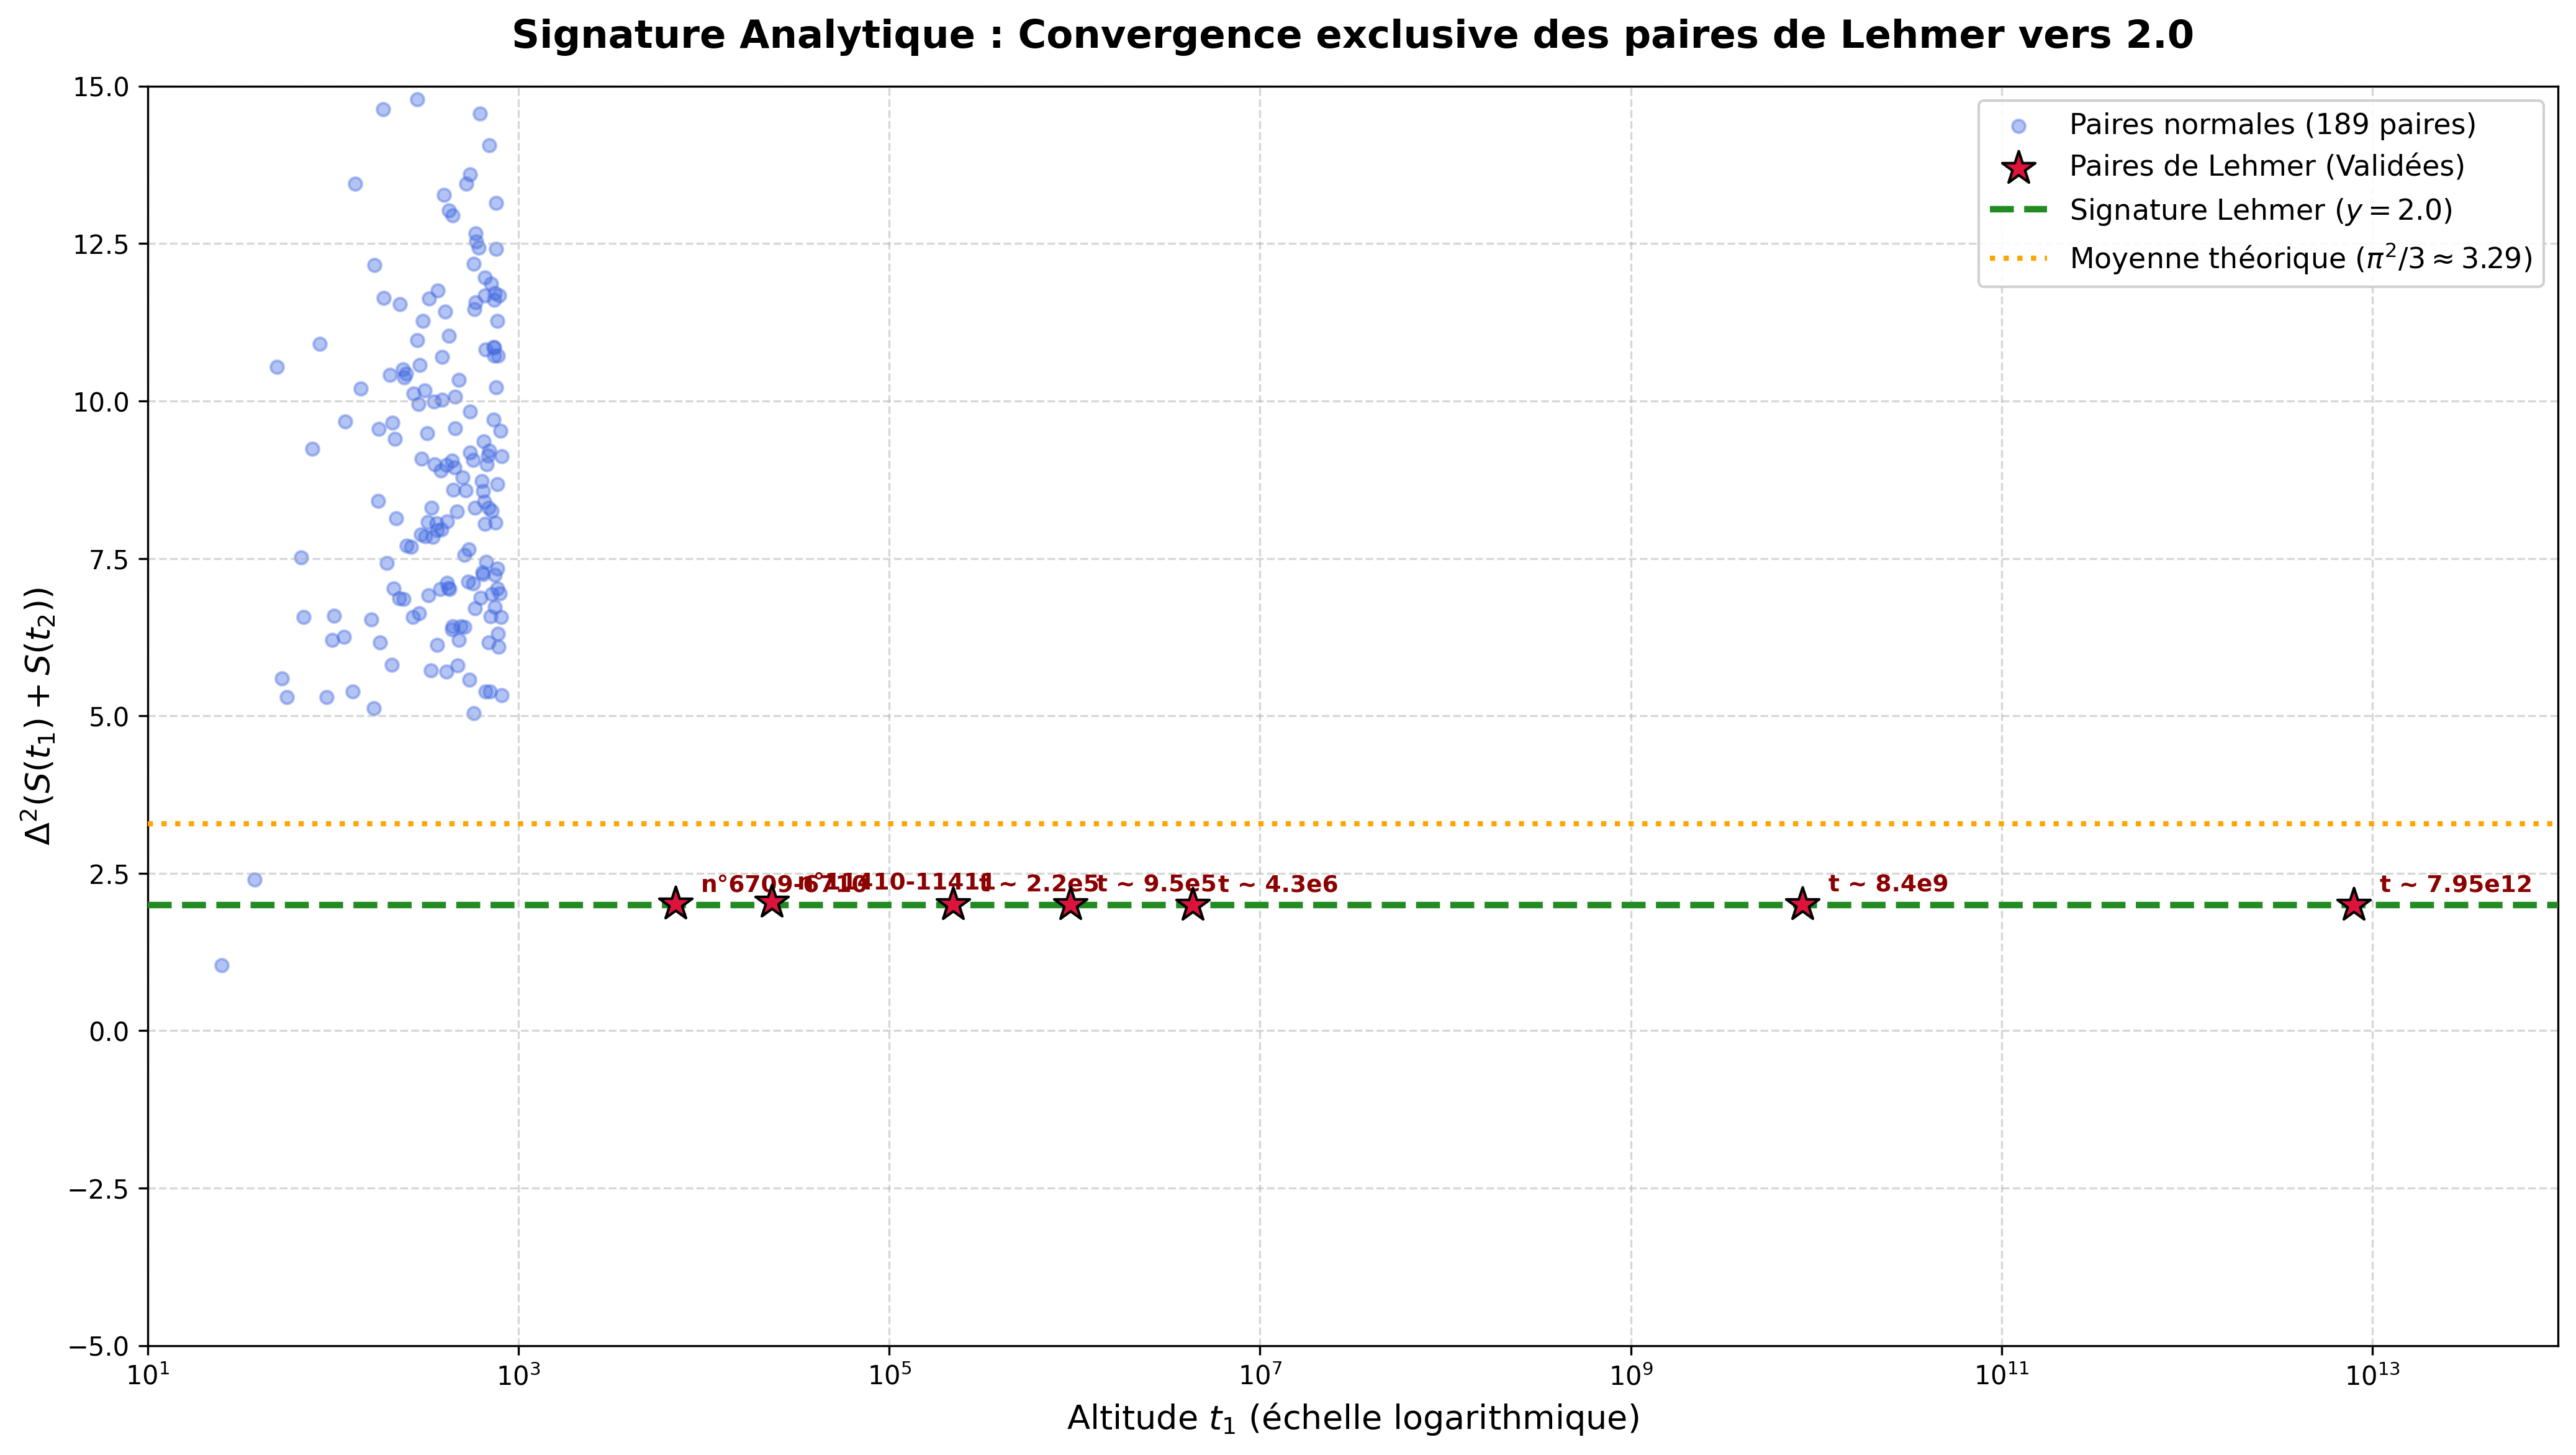
\includegraphics[width=\textwidth]{signature_combinee_lehmer_vs_normal.png}
\caption{Visual comparison of the analytical signature $\Delta^2(S(t_1) + S(t_2))$. The blue cloud represents the normal pairs of the control group, showing high dispersion around the theoretical mean $\pi^2/3 \approx 3.29$ (orange line). The red stars represent the validated Lehmer pairs, which align perfectly on the theoretical line $y = 2$ (dashed green line), independently of the altitude. This clear separation validates the decoupling phenomenon.}
\label{fig:signature_combinee}
\end{figure}

This graph highlights three fundamental facts:
\begin{enumerate}
    \item \textbf{The exclusivity of the signature}: No normal pair converges to the value 2.0.
    \item \textbf{The robustness of the method}: Lehmer pairs align on $y=2$ from $t \approx 7,000$ up to $t \approx 8 \times 10^{12}$.
    \item \textbf{The decoupling phenomenon}: The perfect alignment proves that for Lehmer pairs, the curvature is entirely dominated by the mutual interaction $1/\Delta^2$, isolating them from the rest of the spectrum.
\end{enumerate}

% ============================================================
\section{Conjecture and Conclusion}
% ============================================================

\subsection{The Analytical Signature Conjecture}
Based on the numerical evidence, we propose the following characterization:

\begin{conjecture}[Analytical Signature of Lehmer Pairs]
Let $t_1 < t_2$ be two consecutive zeros of $Z(t)$ on the critical line, with spacing $\Delta = t_2 - t_1$. Let $S(\gamma)$ be the local potential curvature defined in Section~6. The pair $(t_1, t_2)$ is a Lehmer pair if and only if:
\begin{equation}
\boxed{\Delta^2\big(S(t_1) + S(t_2)\big) = 2 + \varepsilon, \quad |\varepsilon| \ll 1}
\end{equation}
\end{conjecture}

\subsection{Conclusion}
This work establishes four major results:
\begin{enumerate}
    \item A \textbf{stable extraction method} for the derivatives of $Z(t)$ via windowed integrals and error-absorbing linear systems, achieving near-machine precision ($10^{-20}$) without axis sweeping.
    \item The validation of a \textbf{local curvature formula} $S(\gamma_n)$ that exactly captures the interaction of the zeros, computable instantaneously without summing over thousands of zeros.
    \item The identification of a \textbf{unique analytical signature} ($\Delta^2(S_1+S_2) \approx 2$) allowing the certification of the ``Lehmer'' nature of a zero pair.
    \item A \textbf{rigorous mathematical explanation} of this signature through a local/global decomposition of the curvature, with an explicit bound $S_{\text{global}}(\gamma_n) \lesssim \frac{\pi^2 - 6}{6\pi} \ln(t/2\pi)$ on the residual term, proving that the decoupling intensifies logarithmically with altitude.
\end{enumerate}

\textbf{Future Perspectives:} The next step is to provide a rigorous proof of the asymptotic equivalence between $S(\gamma_n)$ and the truncated Riemann--von Mangoldt sum, and to use this fast method to map the statistical distribution of the spacings $\Delta$ at medium altitudes ($t \sim 10^5 - 10^6$).

% ============================================================
\section*{Appendix A: Recommended Numerical Parameters}
\addcontentsline{toc}{section}{Appendix A: Recommended Numerical Parameters}
% ============================================================

\begin{table}[h!]
\centering
\begin{tabular}{@{}lccc@{}}
\toprule
\textbf{Altitude $t$} & \textbf{Precision (dps)} & \textbf{$h_1$ recommended} & \textbf{GL Points} \\
\midrule
$< 10^5$ & 50 & $10^{-3}$ & 20 \\
$10^5 - 10^7$ & 60 & $10^{-3}$ & 20 \\
$10^7 - 10^{12}$ & 100 & $\Delta/10$ & 20 \\
$> 10^{12}$ & 100--150 & $\Delta/10$ & 20 \\
\bottomrule
\end{tabular}
\caption{Recommended parameters according to altitude.}
\end{table}

% ============================================================
\section*{Appendix B: Reference Implementation}
\addcontentsline{toc}{section}{Appendix B: Reference Implementation}
% ============================================================
The computations were performed in Python with the \texttt{mpmath} library. Key functions include:
\begin{itemize}
    \item \texttt{A(h, a)}, \texttt{O(h, a)}: windowed integrals,
    \item \texttt{mp.lu\_solve}: for the sponge linear systems,
    \item \texttt{mp.polyroots}: for the 7th-order polynomial,
    \item \texttt{mp.psi(1, z)}: for the trigamma function (analytical computation of $C''/C$).
\end{itemize}

% ============================================================
\section*{Appendix C: Python Code for the Combined Plot}
\addcontentsline{toc}{section}{Appendix C: Python Code for the Combined Plot}
% ============================================================
The following Python script, using the \texttt{pandas} and \texttt{matplotlib} libraries, was used to generate Figure \ref{fig:signature_combinee}. It superimposes the control group data (CSV file) with the validated Lehmer pairs at high altitude.

\begin{verbatim}
import pandas as pd
import matplotlib.pyplot as plt
import numpy as np

# 1. Loading control group data
fichier_csv = 'groupe_temoin_500_paires_20261006_154256.csv'
df = pd.read_csv(fichier_csv)
df_normal = df[df['Est_Normale'] == True]

# 2. Validated Lehmer pairs
lehmer_pairs = [
    {"t1": 7005.062866174921,       "delta2_S": 2.01386, "label": "No. 6709-6710"},
    {"t1": 23153.51496722261,       "delta2_S": 2.04399, "label": "No. 11410-11411"},
    {"t1": 220538.8529632685,       "delta2_S": 2.00431, "label": "t ~ 2.2e5"},
    {"t1": 947107.8201191042,       "delta2_S": 2.01000, "label": "t ~ 9.5e5"},
    {"t1": 4316832.467101349,       "delta2_S": 2.00027, "label": "t ~ 4.3e6"},
    {"t1": 8436151843.542355,       "delta2_S": 2.00929, "label": "t ~ 8.4e9"},
    {"t1": 7954022502373.43289,     "delta2_S": 2.00000, "label": "t ~ 7.95e12"}
]

# 3. Configuration and plotting
fig, ax = plt.subplots(figsize=(14, 8))
ax.scatter(df_normal['t1'], df_normal['Delta2_Somme_S'],
           color='royalblue', alpha=0.4, s=25,
           label=f'Normal pairs ({len(df_normal)} pairs)')

t1_lehmer = [p["t1"] for p in lehmer_pairs]
s_lehmer = [p["delta2_S"] for p in lehmer_pairs]
ax.scatter(t1_lehmer, s_lehmer,
           color='crimson', edgecolor='black', s=180, marker='*',
           zorder=5, label='Lehmer Pairs (Validated)')

for i, txt in enumerate([p["label"] for p in lehmer_pairs]):
    ax.annotate(txt, (t1_lehmer[i], s_lehmer[i]),
                textcoords="offset points", xytext=(10, 5),
                fontsize=9, color='darkred', fontweight='bold')

ax.axhline(y=2.0, color='forestgreen', linestyle='--', linewidth=2.5,
           label='Theoretical Signature ($y = 2.0$)', zorder=4)
ax.axhline(y=np.pi**2/3, color='orange', linestyle=':', linewidth=2,
           label=f'Theoretical mean ($\\pi^2/3 \\approx 3.29$)', zorder=4)

# 4. Formatting
ax.set_xscale('log')
ax.set_xlim(10, 1e14)
ax.set_ylim(-5, 15)
ax.set_xlabel('Altitude $t_1$ (logarithmic scale)', fontsize=13)
ax.set_ylabel('$\\Delta^2 (S(t_1) + S(t_2))$', fontsize=13)
ax.set_title('Analytical Signature: Exclusive convergence of Lehmer pairs to 2.0',
             fontsize=15, fontweight='bold', pad=15)
ax.grid(True, which="both", ls="--", alpha=0.5, zorder=0)
ax.legend(loc='upper right', fontsize=11, framealpha=0.9)

plt.tight_layout()
plt.savefig('signature_combinee_lehmer_vs_normal.png', dpi=300, bbox_inches='tight')
plt.show()
\end{verbatim}

\vspace{1cm}
\begin{center}
\textit{Note written following the numerical validation campaign including the 500-pair control group.}
\end{center}

\end{document}
